%%% LaTeX Template: Two column article
%%%
%%% Source: http://www.howtotex.com/
%%% Feel free to distribute this template, but please keep to referal to http://www.howtotex.com/ here.
%%% Date: February 2011

%%% Preamble
\documentclass[	DIV=calc,%
							paper=a4,%
							fontsize=12pt,%
							onecolumn]{scrartcl}	 					% KOMA-article class
\usepackage[pdftex]{hyperref}
\usepackage{lipsum}													% Package to create dummy text
\usepackage[brazil]{babel}	
\usepackage{scalefnt}
% English language/hyphenation
\usepackage[protrusion=true,expansion=true]{microtype}				% Better typography
\usepackage{amsmath,amsfonts,amsthm}					% Math packages
\usepackage[pdftex]{graphicx}									% Enable pdflatex
\usepackage[svgnames]{xcolor}									% Enabling colors by their 'svgnames'
\usepackage[hang, small,labelfont=bf,up,textfont=it,up]{caption}	% Custom captions under/above floats
\usepackage{epstopdf}												% Converts .eps to .pdf
\usepackage{subfig}													% Subfigures
\usepackage{booktabs}												% Nicer tables
\usepackage{fix-cm}													% Custom fontsizes
\usepackage[utf8]{inputenc}
\usepackage[top=2.5cm, bottom=2.5cm, left=2.5cm, right=2.5cm]{geometry}
\usepackage[ddmmyyyy]{datetime}
\addto\captionsenglish{%
	\renewcommand\tablename{Tabela}
	\renewcommand\figurename{Figura}
} 
 

 
%%% Custom sectioning (sectsty package)
\usepackage{sectsty}													% Custom sectioning (see below)
\allsectionsfont{%															% Change font of al section commands
	\usefont{OT1}{phv}{b}{n}%										% bch-b-n: CharterBT-Bold font
	}

\sectionfont{%																% Change font of \section command
	\usefont{OT1}{phv}{b}{n}%										% bch-b-n: CharterBT-Bold font
	}



%%% Headers and footers
\usepackage{fancyhdr}												% Needed to define custom headers/footers
	\pagestyle{fancy}														% Enabling the custom headers/footers
\usepackage{lastpage}	
\usepackage{lscape}
% Header (empty)
\lhead{}
\chead{}
\rhead{}
% Footer (you may change this to your own needs)

%% ====================================
%% ====================================
%% mude o rodape  do projeto
%% ====================================
%% ====================================

\lfoot{\footnotesize \texttt{Processo Unificado Adaptado} \textbullet Gerenciamento de Configuração}


\cfoot{}
\rfoot{\footnotesize página \thepage\ de \pageref{LastPage}}	% "Page 1 of 2"
\renewcommand{\headrulewidth}{0.0pt}
\renewcommand{\footrulewidth}{0.4pt}



%%% Creating an initial of the very first character of the content
\usepackage{lettrine}
\newcommand{\initial}[1]{%
     \lettrine[lines=3,lhang=0.3,nindent=0em]{
     				\color{DarkGoldenrod}
     				{\textsf{#1}}}{}}



%%% Title, author and date metadata
\usepackage{titling}															% For custom titles

\newcommand{\HorRule}{\color{DarkGoldenrod}%			% Creating a horizontal rule
									  	\rule{\linewidth}{1pt}%
										}

\pretitle{\vspace{-30pt} \begin{flushleft} \HorRule 
				\fontsize{50}{50} \usefont{OT1}{phv}{b}{n} \color{DarkRed} \selectfont 
				}

%% ====================================
%% ====================================
%% mude o titulo  do projeto
%% ====================================
%% ====================================

\title{Modelo incremental adaptado }					% Title of your article goes here

%% ====================================



\posttitle{\par\end{flushleft}\vskip 0.5em}

\preauthor{\begin{flushleft}
					\large \lineskip 0.5em \usefont{OT1}{phv}{b}{sl} \color{DarkRed}}
\author{Erik Henrique de Oliveira, Vitor Padiar Carnevalli, João Pirolo }  	% Author name goes here


\postauthor{\footnotesize \usefont{OT1}{phv}{m}{sl} \color{Black} 
					\\Universidade Tecnológica Federal do Paraná - Campus Cornélio Procópio 								% Institution of author
					\par\end{flushleft}\HorRule}

\date{}																				% No date




%%% Begin document
\begin{document}
\maketitle
\thispagestyle{fancy} 	
\thispagestyle{empty}		% Enabling the custom headers/footers for the first page 
% The first character should be within \initial{}




%% ====================================
%% ====================================
%% mude o resumo  do projeto
%% ====================================
%% ====================================
\initial{E}\textbf{este trabalho apresenta uma adaptação dos processos incremental e unificado, onde um grupo de três Eng. de Software trabalhão no processo de desenvolvimento de um produto comercial de software. } 

%% ====================================
\begin{figure}
	\centering
	
\includegraphics{utfpr}
\end{figure}

\vspace{3cm}
\centerline{\textit{\textbf{\today}}}

\clearpage
    \renewcommand*\listfigurename{Lista de figuras}
\listoffigures

\renewcommand*\listtablename{Lista de tabelas}
\listoftables




\clearpage
\renewcommand{\contentsname}{Sumário}
\tableofcontents
\clearpage

%% ====================================
%% ====================================
%% Inicio do texto
%% ====================================
%% ====================================
\section{Introdução}

O desenvolvimento de um software é uma grande tarefa que pode ser estendida por vários meses, possivelmente até um ano ou mais. Para tornar esta tarefa mais rápida e pratica é importante, dividir o trabalho em partes menores ou iterações. Cada iteração resultará num incremento ou uma versão de software. 

 Iterações são passos do fluxo de trabalho e incrementos são crescimentos do produto.

O princípio do processo incremental e iterativo é que, a equipe envolvida, possa refinar e aumentar, aos poucos, a qualidade, os requisitos até atingir o sistema final.  Isso faz toda a diferença, quando falamos em grandes sistemas, a serem automatizados.   

Como o processo teve de ser adaptado a um grupo pequeno ele sofreu algumas alterações principalmente na fase de construção e transição, a nomenclatura adotada para esse modelo de processo foi: Processo Ágil Incremental adaptado.

O processo foi desenvolvido pelos desenvolvedores:
\begin{itemize}
{\item João Pirolo - Github: https://github.com/JoaoPirolo,
\item Erik Zambeli - gitHub: https://github.com/ErikZA, 
\item Vitor Padiar - GitHub: https://github.com/vitorpadiar.}
\end{itemize} 
\section{Processo}

 O Processo Unificado surgiu como um processo para o desenvolvimento de software orientados a objetos. É um processo iterativo e adaptativo de desenvolvimento que devido a maneira organizada e consistente permite conduzir um projeto de sua concepção a sua implantação.
 
 O PU utiliza um paradigma evolucionário paro o desenvolvimento de softwares. O ciclo de vida iterativo é baseado em versões e incrementos sucessivos a fim de integrar um sistema adequado. Em cada iteração incrementa-se um pouco mais o produto, baseando-se na experiência obtida nas iterações anteriores e no feedback do usuário. Cada iteração pode ser considerada uma nova versão do software de duração fixa, sendo que cada uma destas inclui suas próprias atividades de análise de requisitos, projeto, implementação e testes.
 
  Em cada iteração é escolhido um pequeno subconjunto de requisitos, os quais são rapidamente projetados, implementados e testados pelos usuários. Isso leva a uma realimentação rápida de requisitos baseada em dados concretos de usuários, desenvolvedores e testes, o PU prega uma atitude de aceitar a mudança e a adaptação como fatores inevitáveis e essenciais. Não se deve tentar especificar completamente o sistema em uma tacada interação só, essa ideia cria um conjunto congelado de requisitos.
 
 O resultado de cada iteração é um sistema executável, porém incompleto. Ele não está pronto para ser colocado em produção e pode continuar nesta situação ainda por muitas iterações mais cada iteração produz um sistema com qualidade de produto final, e não somente um protótipo.
 
  Modelo de processo unificado figura \ref{rup1}: 
 \begin{figure}
	\centering
	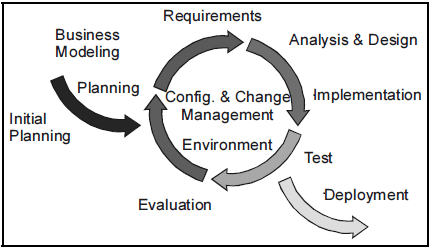
\includegraphics[]{rup1.png}
	\caption{Exemplo de Modelo Unificado}
	\label{rup1}
\end{figure}
 
 O Processo Unificado organiza suas iterações em quatro fases principais:
\begin{itemize}

\item Concepção: o objetivo desta fase é levantar, de forma genérica e pouco precisa, o escopo do projeto. Não deve existir aqui a pretensão de especificar de forma detalhada requisitos, a ideia é ter uma visão inicial do problema, estimar de forma vaga esforço e prazos e determinar se o projeto é viável e merece uma análise mais profunda.

\item Elaboração: na fase de elaboração todos (ou a grande maioria dos requisitos) são levantados em detalhes. Numa primeira iteração um ou dois requisitos, os de maior risco e valor arquitetural, são especificados em detalhes. Estes são implementados e servem como base de avaliação junto ao usuário e desenvolvedores para o planejamento da próxima iteração. Em cada nova iteração os requisitos antigos são melhor esclarecidos e novos são detalhados. Ao fim da fase, com os requisitos levantados em detalhes, os principais riscos foram tratados e pode-se então fazer estimativas mais realistas.

\item Construção: implementação iterativa dos elementos restantes de menor risco e mais fáceis e preparação para a implantação.

\item Transição: testes finais e implantação.

\end{itemize}

O Processo Unificado foi criado para ser um processo ágil de desenvolvimento e prega uma abordagem realística para a condução de um projeto. Para a sua utilização durante o desenvolvimento devido ao pequeno grupo tivemos de adaptar e modificar as atividades de suas fases para atender as necessidades do desenvolvimento.

\subsection{Papeis}

O processo original exigia a demanda de muitos papeis, para facilitar a adaptação do processo e a melhor distribuição das atividades, adotamos os seguintes papeis para nossa organização:

\begin{itemize}

	\item Gerente de Projeto e configuração: Descreve os objetivos do projeto e como ele será realizado. Inclui estimativas de custo e programação trata da identificação das atividades a serem realizadas, os artefatos e os documentos a serem produzidos, versões a serem entregues, realiza o levantamento do custo do projeto, em um segundo release acompanha o projeto de forma constante verificando o progresso e os custos  comparando com o que foi planejado inicialmente, elaboração de relatórios prestação de contas e de resultados. Ainda atua como gerente de configuração controla o processo de gestão de configuração, sendo responsável pelas bases de itens de configuração e de requisições de mudança. Assim, ele controla a entrada e a saída de dados nessas bases, bem como autoriza, ou não, possíveis alterações, a fim de manter a integridade dos itens de configuração e das baselines.

	\item Analista de Sistema: levantamentos de requisitos e regras de negócio, mapeamento dos processos elaboração dos casos de uso baseado nos requisitos dos clientes, garantia da integridade dos sistemas, realizar o planejamento das versões, atua também como analista de implantação elaborando o plano de implantação da aplicação e coleta requisitos necessários para as próximas versões, aplica treinamento aos usuários.

	\item Desenvolvedor: Desenvolver, testar e liberar versões para a implantação e manter os sistemas de acordo com metodologia e técnicas propostas, para garantir a qualidade, o custo e prazo. E raliza auditorias nos codigos assim como verifica se as metricas estabelecidas foram atendidas.
\end{itemize}  
\subsection{Atividades}
\begin{itemize}
\item Atividades do Desenvolvedor tabela \ref{tab3}:
\begin{table}[h!]
\centering
\caption{Tabela tarefas do Desenvolvedor}
\label{tab3}
\begin{tabular}{|l|l|l|}
\hline
\begin{tabular}[c]{@{}l@{}}Item /\\  papel\end{tabular} & Desenvolvedor                                                        & Aplicações                                                                                                                                                                                                                                                                       \\\hline
1                                                       & \begin{tabular}[c]{@{}l@{}}Desenvolver\\  o código\end{tabular}      & \begin{tabular}[c]{@{}l@{}}A atividade de desenvolver incremento de software consiste \\ em escrever o código-fonte que implementa, \\ ou corrige, um ou mais requisitos do software. \\ Esta atividade pode ser \\ realizada mais de uma vez durante uma iteração.\end{tabular} \\\hline
2                                                       & \begin{tabular}[c]{@{}l@{}}Realizar teste \\ de Unidade\end{tabular} & \begin{tabular}[c]{@{}l@{}}Trata-se de um teste do tipo estrutural \\ (caixa-branca) que deve ser produzido pelo \\ programador, em parceria com o testador, antes da \\ implementação da unidade de software.\end{tabular}                                                      \\\hline
3                                                       & \begin{tabular}[c]{@{}l@{}}Corrigir \\ Bugs\end{tabular}             & \begin{tabular}[c]{@{}l@{}}Avaliar os resultados positivos \\ e negativos dos testes.\end{tabular}                                                                                                                                                                               \\\hline
4                                                       & \begin{tabular}[c]{@{}l@{}}Integração \\ do Software\end{tabular}    & \begin{tabular}[c]{@{}l@{}}desenvolver o sistema dividindo-o em módulos ou componentes, \\  funcionalidades do componente integrado devem \\ funcionar corretamente no sistema produzido.\end{tabular}                                                                           \\\hline
5                                                       & \begin{tabular}[c]{@{}l@{}}Teste de \\ Aceitação\end{tabular}        & \begin{tabular}[c]{@{}l@{}}Nesta etapa devem ser executados os testes de sistema e, \\ se aplicáveis, os testes de aceitação.\end{tabular}                                                                                                                                       \\\hline
6                                                       & \begin{tabular}[c]{@{}l@{}}Liberação \\ da Versão\end{tabular}       & \begin{tabular}[c]{@{}l@{}}Liberar uma versão testada \\ e atualizada do Incremento\end{tabular}                                                                           \\\hline                  7                                                       & \begin{tabular}[c]{@{}l@{}}Auditoria \\ e Medição\end{tabular}       & \begin{tabular}[c]{@{}l@{}}são realizadas objetivamente para
assegurar que as baselines\\ e os itens de configuração estejam
íntegros,\\ completos e consistentes. \end{tabular}                                                                           \\\hline                                                                                    
\end{tabular}
\end{table}
\item Atividades do Gerente Projetos e Configuração tabela \ref{tab1}:
\begin{landscape}
\begin{table}[h!]
\scalefont{0.8}
\caption{Tabela tarefas do Gerente de Projetos e Configuração}
\label{tab1}
\begin{tabular}{|l|l|l|}
\hline
\begin{tabular}[c]{@{}l@{}}Item / \\ papel\end{tabular} & Gerente de Projetos & Aplicações \\ \hline
1 & Elaborar Termo de Abertura do Projeto & Formaliza o inicio do Projeto \\ \hline
2 & Monitoramento e Controle & Assegurar que objetivos sejam atingidos \\ \hline
3 & -Controle de Qualidade & Definir padrões em procedimentos, políticas e ações, de maneira uniforme. \\ \hline
4 & -Validar o Escopo & Processo de formalizar a aceitação das entregas do projeto. \\ \hline
5 & -Controlar o Escopo & Controlar as entregas do Projeto \\ \hline
6 & -Controlar os Riscos & \begin{tabular}[c]{@{}l@{}}Acompanhar os riscos identificados; Implementar os planos de respostas aos riscos; Monitorar os riscos \\residuais; Identificar novos riscos; Avaliar a eficácia do processo de riscos durante o ciclo de vida do projeto.\end{tabular} \\ \hline
7 & -Controlar o Cronograma & \begin{tabular}[c]{@{}l@{}}Atualizar o progresso do projeto, monitorar as variações entre o real com o planejado (linha de base) \\ e gerenciar as mudanças ocorridas.\end{tabular} \\ \hline
8 & -Controlar os Custos & Monitorar o status do projeto para atualizar o orçamento e gerenciar alterações na linha de base dos custos. \\ \hline
9 & Identificar Partes Interesadas & \begin{tabular}[c]{@{}l@{}}Processo de identificação de todas as pessoas ou organizações que podem ser afetadas pelo projeto e \\ documentação das informações relevantes relacionadas \\ aos seus interesses, envolvimento e impacto no sucesso do projeto.\end{tabular} \\ \hline
10 & Atualização  da TAP envio para o cliente & \begin{tabular}[c]{@{}l@{}}O termo de abertura do projeto deve conter informações sumarizadas porém com o nível de \\ detalhamento necessário para a aprovação ou não do projeto.\end{tabular} \\ \hline
11 & Encerramento do Projeto & \begin{tabular}[c]{@{}l@{}}Quando o projeto é encerrado o gerente de projeto deve finalizar todos relatórios, \\documentar a experiência do projeto, fornecer informação sobre o produto do projeto \\ e como atendeu seus requisitos do projeto, e então, documentar as lições aprendidas.\end{tabular} \\ \hline
12 & Escopo do Projeto & \begin{tabular}[c]{@{}l@{}}Trabalho que precisa ser realizado para entregar um produto, serviço ou resultado \\ com as características e funções especificadas\end{tabular} \\ \hline
13 & Elaboração do Plano de Gerenciamento de Versões & gerenciar diferentes versões no desenvolvimento do software e do documento \\ \hline
14 & Planejamento da Versão & \begin{tabular}[c]{@{}l@{}}planejar a versão do produto para a entrega, estabelecendo um plano e a meta que o \\Time e o resto da organização possam entender e comunicar.\end{tabular} \\ \hline
15 & Revisão Planejamento e Refinamento & Essa tarefa compreende o planejamento da homologação e a revisão geral do Plano de Projeto. \\ \hline
16 & Gerenciar Comunicação & \begin{tabular}[c]{@{}l@{}}é o processo de colocar as informações necessárias à disposição das partes interessadas no projeto \\ conforme planejado.\end{tabular} \\ \hline
17 & Mobilizar Equipes & tem como objetivo obter os recursos humanos necessários para o projeto. \\ \hline
18 & \begin{tabular}[c]{@{}l@{}}Formalizar \\ Encerramento\end{tabular} & \begin{tabular}[c]{@{}l@{}}Gerar o documento de encerramento, coletando assinatura das partes, \\ registrar pontos fortes e fracos do desenvolvimento.\end{tabular} \\ \hline
19 & \begin{tabular}[c]{@{}l@{}}Identificar Produtos\\ Reusaveis\end{tabular} & identificar e catalogar os produtos de software do projeto que podem ser reusados em outros projetos \\ \hline
20 & Registrar Base Histórica & \begin{tabular}[c]{@{}l@{}}conjunto de lições aprendidas deve ser compilado juntamente com os registros de\\ alterações da execução do projeto em relação ao planejamento.\end{tabular} \\ \hline
21 & Criar Baseline & \begin{tabular}[c]{@{}l@{}}conjunto de itens de configuração que, normalmente, representa o estado de desenvolvimento dos artefatos \\ do projeto em um determinado momento.\end{tabular} \\ \hline
22 & \begin{tabular}[c]{@{}l@{}}Adicionar Itens de \\ Configuração\end{tabular} & \begin{tabular}[c]{@{}l@{}}Os artefatos validados (novos ou alterados) que compõem a baseline devem ser inseridos \\ na base de itens de configuração.\end{tabular} \\ \hline
23 & Arquivar Baseline & arquivar a baseline anterior no Sistema de Gestão de Configuração. \\ \hline
24 & Liberar Baseline & disponibilizar a baseline para uso no Sistema de Gestão de Configuração. \\ \hline
\end{tabular}
\end{table}
\end{landscape}
\item Atividades do Analista de Sistemas tabela \ref{tab2}:
\begin{table}[h!]
\caption{Tabela tarefas do Analista de sistemas}
\label{tab2}
\begin{tabular}{|l|l|l|}
\hline
\begin{tabular}[c]{@{}l@{}}Item / \\ papel\end{tabular} & \begin{tabular}[c]{@{}l@{}}Analista de \\ Sistemas\end{tabular}                 & Aplicações                                                                                                                                                                                                                                                                              \\\hline
1                                                       & \begin{tabular}[c]{@{}l@{}}Construir Modelo\\  de Dominio\end{tabular}          & \begin{tabular}[c]{@{}l@{}}Esta tarefa compreende a definição do\\  modelo de Dominio de alto nível.\end{tabular}                                                                                                                                                                       \\
2                                                       & \begin{tabular}[c]{@{}l@{}}Construir Modelo\\  de Negócio\end{tabular}          & \begin{tabular}[c]{@{}l@{}}Consiste em construir um \\ modelo do negocio de alto nivel.\end{tabular}                                                                                                                                                                                    \\\hline
3                                                       & \begin{tabular}[c]{@{}l@{}}Construir Casos de \\ Uso de Alto Nível\end{tabular} & \begin{tabular}[c]{@{}l@{}}Consiste em construir \\ casos de uso de alto nivel\end{tabular}                                                                                                                                                                                             \\\hline
4                                                       & \begin{tabular}[c]{@{}l@{}}Elaborar \\ casos de Teste\end{tabular}              & \begin{tabular}[c]{@{}l@{}}A elaboração dos casos de testes devem \\ objetivar a identificação dos erros \\ que eventualmente existam no sistema.\\  Além disso, tais documentos \\ servem como insumo para a verificação \\ se todos os requisitos estão sendo atendidos.\end{tabular} \\\hline
5                                                       & \begin{tabular}[c]{@{}l@{}}Prototipar a Interface \\ com o Usuário\end{tabular} & \begin{tabular}[c]{@{}l@{}}Desenvolver interfaces de fácil \\ intendimento para ajudar na coleta \\ de requisitos e no desenvolvimento do inclemento.\end{tabular}                                                                                                                      \\\hline
6                                                       & \begin{tabular}[c]{@{}l@{}}Treinar \\ Usuários\end{tabular}                     & \begin{tabular}[c]{@{}l@{}}Assim que liberada a versão deve apresentar ao usuário, \\ para que o mesmo faça a validação no treinamento.\end{tabular}                                                                                                                                    \\\hline
7                                                       & \begin{tabular}[c]{@{}l@{}}Revisão e \\ novos requisitos\end{tabular}           & \begin{tabular}[c]{@{}l@{}}Detalhar requisitos funcionais restantes. \\ Esse detalhamento é realizado em \\ conjunto com o Cliente e resulta na criação \\ de um documento de Requisitos\end{tabular}                                                                                   \\\hline
8                                                       & Implantação                                                                     & \begin{tabular}[c]{@{}l@{}}A implantação do sistema consiste da \\ entrega do produto final para o cliente. \\ Sendo necessário para isso a criação do \\ ambiente no qual o sistema será executado.\end{tabular} \\\hline

\end{tabular}
\end{table}
\end{itemize}

\section{Conjunto de normas}

\subsection{MPS.BR – Melhoria de Processo de Software}
O aumento da competitividade faz com que as organizações busquem a qualidade dos produtos de software e serviços, além dos processos de produção e distribuição. Dessa forma a qualidade é um fator de alta criticidade para o sucesso na indústria de software.
No Brasil há um baixo investimento das empresas na busca dos certificados de qualidade, isso se devido ao alto investimento que deve ser movimentado para certificações que comprovem a qualidade e a maturidade dos processos, deixando de fora médias e pequenas organizações que não possuem recursos suficientes para investir.
Por tais motivos para este processo utilizamos o MPS. BR, coordenado pela Associação para Promoção da Excelência do Software Brasileiro (SOFTEX), que visa tornar os softwares brasileiros compatíveis com os padrões de qualidades que são exigidos internacionalmente, tendo como foco em micro, pequenas e médias empresas.

As metas do Programa MPS.BR são:
\begin{itemize}
    \item Criação e aprimoramento de um modelo para melhoria e avaliação dos processos e serviços; Capacitação de pessoas através de programas de treinamento, à um custo viável; Credenciamento de Instituições Implementadoras (II) e Avaliadoras (IA);
    
    \item Criação e aprimoramento de um Modelo de Negócio para Melhoria de Processo de Software (MN-MPS); Implementação do modelo MPS em empresas de micro, pequeno e médio porte a um custo viável; Avaliação do modelo nas organizações a um custo viável.
\end{itemize}

O modelo MPS possui três componentes: Modelo de Referência para Melhoria de Processo de Software (MR-MPS), Método de Avaliação para Melhoria de Processo de Software (MA-MPS) e Modelo de Negócio para Melhoria de Processo de Software (MN-MPS).

Ramificação do processo MPS'Br figura \ref{rup4}: 
 \begin{figure}[h!]
	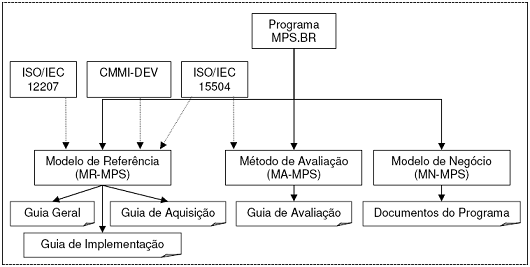
\includegraphics[scale=0.8]{ArvoreMPS.png}
	\caption{Ramificação do processo MPS'Br}
	\label{rup4}
\end{figure}

MR-MPS (Modelo de Referência para Melhoria do Processo de Software)
O Modelo de Referência possui os requisitos que os processos das unidades organizacionais devem atender para está de acordo com o MPS (SOFTEX, 2012). O MR-MPS é definido por níveis de maturidade, sequenciais e acumulativos. Cada um dos níveis de maturidade é composto por um conjunto de processos em um determinado nível de capacidade (WEBER, ARAÚJO, et al., 2006). Um nível de maturidade é atingido quando os seus resultados, propósitos do processo e atributos relacionados aos processos são atendidos.
O MR-MPS define sete níveis de maturidade: A (Em Otimização), B (Gerenciado Quantitativo), C (Definido), D (Largamente Definido), E (Parcialmente Definido), F (Gerenciado) e G (Parcialmente Gerenciado). O nível G é considerado o mais imaturo entre os demais e o A o mais maduro. Esses níveis possui um paralelo com os quatro níveis de maturidade dos estágios definidos pelo CMMI – Capability Maturity Model Integration (de 2 a 5).
Níveis de Maturidade MPS'Br figura \ref{rup2}: 
 \begin{figure}[h!]
	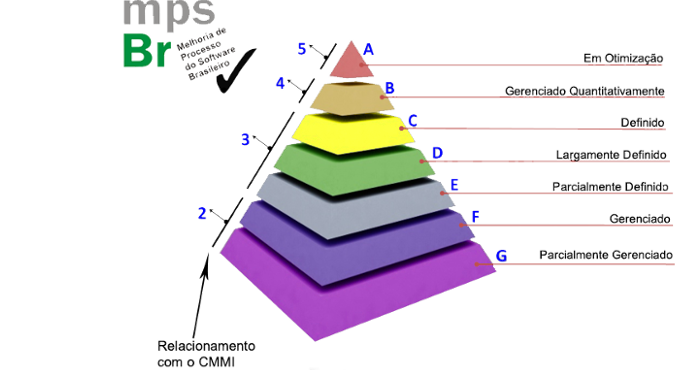
\includegraphics[scale=2.8]{mpsbr.png}
	\caption{Níveis de Maturidade MPS'Br}
	\label{rup2}
\end{figure}

\subsection{MPS'Br Nível de maturidade F}
    O projeto apresenta caracteristicas, como os níveis de maturidade que permitem uma implementação de forma gradual e adequada a realidade das micro, pequenas e médias organizações, além disso, é um modelo totalmente adaptado a realidade brasileira, compatíveis com as normas ISO/IEC 12207, ISO/IEC 155504 e CMMI.

Como a experiencia da equipe no desenvolvimento de softwares e no trabalho com o modelo de processo apresentado ainda e prematuro tentamos adotar o nível de maturidade F (Gerenciado) para alcançá-lo devemos implementar os processos do nível de maturidade G (Parcialmente Gerenciado) e ainda evoluir adotandos os processos do nível F.

A seguir a descrição detalhada dos resultados esperados do processo:
\begin{itemize}
\item[1]{\textbf{Gerência de Projetos – GPR}}

\item GPR 1. O escopo do trabalho para o projeto é definido; 
\item GPR 2. As tarefas e os produtos de trabalho do projeto são dimensionados utilizando métodos apropriados; 
\item GPR 3. O modelo e as fases do ciclo de vida do projeto são definidos; 
\item GPR 4. (Até o nível F) O esforço e o custo para a execução das tarefas e dos produtos de trabalho são estimados com base em dados históricos ou referências técnicas; 
\item GPR 4. (A partir do nível E) O planejamento e as estimativas das tarefas do projeto são feitos baseados no repositório de estimativas e no conjunto de ativos de processo organizacional; 
\item GPR 5. O orçamento e o cronograma do projeto, incluindo a definição de marcos e pontos de controle, são estabelecidos e mantidos;
\item GPR 6. Os riscos do projeto são identificados e o seu impacto, probabilidade de ocorrência e prioridade de tratamento são determinados e documentados; 
\item GPR 7. Os recursos humanos para o projeto são planejados considerando o perfil e o conhecimento necessários para executá-lo; 
\item GPR 8. (Até o nível F) Os recursos e o ambiente de trabalho necessários para executar o projeto são planejados; 
\item GPR 9. Os dados relevantes do projeto são identificados e planejados quanto à forma de coleta, armazenamento e distribuição. Um mecanismo é estabelecido para acessá-los, incluindo, se pertinente, questões de privacidade e segurança; 
\item GPR 10. Um plano geral para a execução do projeto é estabelecido com a integração de planos específicos; 
\item GPR 11. A viabilidade de atingir as metas do projeto é explicitamente avaliada considerando restrições e recursos disponíveis. Se necessário, ajustes são realizados; 
\item GPR 12. O Plano do Projeto é revisado com todos os interessados e o compromisso com ele é obtido e mantido; 
\item GPR 13. O escopo, as tarefas, as estimativas, o orçamento e o cronograma do projeto são monitorados em relação ao planejado; 
\item GPR 14. Os recursos materiais e humanos bem como os dados relevantes do projeto são monitorados em relação ao planejado; 
\item GPR 15. Os riscos são monitorados em relação ao planejado; 
\item GPR 16. O envolvimento das partes interessadas no projeto é planejado, monitorado e mantido; 
\item GPR 17. Revisões são realizadas em marcos do projeto e conforme estabelecido no planejamento; 
\item GPR 18. Registros de problemas identificados e o resultado da análise de questões pertinentes, incluindo dependências críticas, são estabelecidos e tratados com as partes interessadas; 
\item GPR 19. Ações para corrigir desvios em relação ao planejado e para prevenir a repetição dos problemas identificados são estabelecidas, implementadas e acompanhadas até a sua conclusão; 

\item[2] {\textbf{Gerência de Requisitos – GRE}}

\item GRE 1. O entendimento dos requisitos é obtido junto aos fornecedores de requisitos; 
\item GRE 2. Os requisitos são avaliados com base em critérios objetivos e um comprometimento da equipe técnica com estes requisitos é obtido; 
\item GRE 3. A rastreabilidade bidirecional entre os requisitos e os produtos de trabalho é estabelecida e mantida; 
\item GRE 4. Revisões em planos e produtos de trabalho do projeto são realizadas visando identificar e corrigir inconsistências em relação aos requisitos; 
\item GRE 5. Mudanças nos requisitos são gerenciadas ao longo do projeto.


\item[3] {\textbf{Aquisição – AQU}}
\item Conforme seção 8.4 do MPS’Br – 2012 paragrafo 2: 
“É permitida a exclusão completa do seguinte processo, desde que não executado pela organização: 
Aquisição (AQU)”

\item[4] {\textbf{Gerência de Configuração – GCO}}

\item GCO 1. Um Sistema de Gerência de Configuração é estabelecido e mantido; 
\item GCO 2. Os itens de configuração são identificados com base em critérios estabelecidos; 
\item GCO 3. Os itens de configuração sujeitos a um controle formal são colocados sob baseline; GCO 4. A situação dos itens de configuração e das baselines é registrada ao longo do tempo e disponibilizada; 
\item GCO 5. Modificações em itens de configuração são controladas; 
\item GCO 6. O armazenamento, o manuseio e a liberação de itens de configuração e baselines são controlados; 
\item GCO 7. Auditorias de configuração são realizadas objetivamente para assegurar que as baselines e os itens de configuração estejam íntegros, completos e consistentes.

\item[5] {\textbf{Garantia da Qualidade – GQA}}

\item GQA 1. A aderência dos produtos de trabalho aos padrões, procedimentos e requisitos aplicáveis é avaliada objetivamente, antes dos produtos serem entregues e em marcos predefinidos ao longo do ciclo de vida do projeto; 
\item GQA 2. A aderência dos processos executados às descrições de processo, padrões e procedimentos é avaliada objetivamente; 
\item GQA 3. Os problemas e as não-conformidades são identificados, registrados e comunicados; 
\item GQA 4. Ações corretivas para as não-conformidades são estabelecidas e acompanhadas até as suas efetivas conclusões. Quando necessário, o escalamento das ações corretivas para níveis superiores é realizado, de forma a garantir sua solução;

\item[6] {\textbf{Gerência de Portfólio de Projetos – GPP}}

\item Conforme seção 8.4 do MPS’Br – 2012 paragrafo 3: 
"É permitida a exclusão completa do seguinte processo, desde que a única atividade
da unidade organizacional seja evolução de produto:
Gerência de Portfólio de Projetos (GPP) "

\item[7] {\textbf{Medição – MED}}
\item MED 1. Objetivos de medição são estabelecidos e mantidos a partir dos objetivos de negócio da organização e das necessidades de informação de processos técnicos e gerenciais; 
\item MED 2. Um conjunto adequado de medidas, orientado pelos objetivos de medição, é identificado e definido, priorizado, documentado, revisado e, quando pertinente, atualizado; 
\item MED 3. Os procedimentos para a coleta e o armazenamento de medidas são especificados; 
\item MED 4. Os procedimentos para a análise das medidas são especificados; 
\item MED 5. Os dados requeridos são coletados e analisados; 
\item MED 6. Os dados e os resultados das análises são armazenados; 
\item MED 7. Os dados e os resultados das análises são comunicados aos interessados e são utilizados para apoiar decisões.
\end{itemize}

\section{Execução do porcesso valores e praticas MPS'Br}
\subsection{Gerenciamento de progetos GPR}

Atraves das praticas apresentadas busca-se atingir os 19 resultados esperados no GPR.

O proposito do processo Gerencia de Projetos é estabelecer e manter planos é estabelecer e manter planos que definam as atividades, recursos e responsabilidades do projeto, bem como prover informações sobre o andamento do projeto que permita a realização da correção quando houver desvios significativos no desempenho do projeto.
Definição do escopo do projeto: Após identificar as partes interessadas que serão atendidas no projeto, a próxima preocupação deve ser o escopo, o que será feito no projeto. Uma definição de escopo mal feita implicará em um projeto mal sucedido. O escopo e principalmente a EAP, será a base para os outros processos das outras áreas de conhecimento. Para cada pacote de trabalho da EAP, será definida as atividades necessárias para sua execução (prazo) e posteriormente, os recursos necessários para determinar o orçamento do projeto (custo), e assim por diante.

{\textbf{Estimativas e orçamentação:}} A estimativa de custos deve ser feita com muito cuidado e com o maior nível de detalhes possível. São esses números que irão determinar se o projeto será viável ou não do ponto de vista econômico e financeiro. Na etapa, "Planejamento dos recursos", já foi feita a identificação dos recursos necessários para a realização do projeto. Cabe, agora, para cada item relacionado, estimar seu custo. O ideal é buscar o preço de cada item e mão de obrai na base histórica. Porém, nem sempre isso é possível ou viável. Quando isso não pode ser feito, lança-se mão de índices e estatísticas confiáveis, de projetos semelhantes e de analogias.

{\textbf{Criação do cronograma:}} Desenvolver o Cronograma envolve analisar a sequência das atividades, sua duração, seus requerimentos de recursos e suas restrições para criar o cronograma do projeto e determinar as datas de início e término de cada atividade. É um processo interativo que consolida os processos:

•	Definir as atividades

•	Sequenciar as atividades

•	Estimar os recursos das atividades

•	Estimar as durações das atividades.

{\textbf{Gerenciamento dos riscos: }}Segundo o Guia PMBOK®, o gerenciamento dos riscos do projeto inclui os processos de planejamento, identificação, análise, planejamento de respostas, monitoramento e controle de riscos de um projeto. Seu objetivo é maximizar a exposição aos eventos positivos e minimizar a exposição aos eventos negativos.


Gerenciamento e identificação dos riscos \ref{rup5}: 
 \begin{figure}[h!]
    \centering
	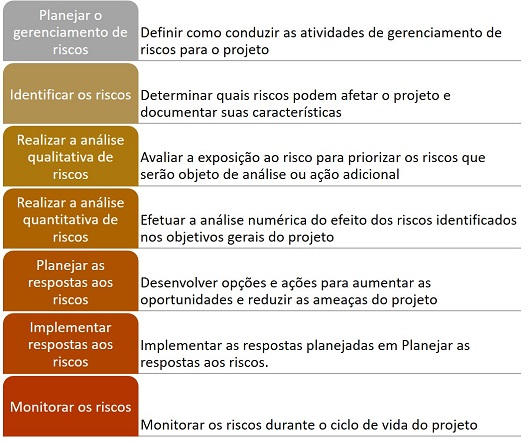
\includegraphics[scale=1.5]{gerenciamento-dos-riscos.jpg}
	\caption{Gerenciamento dos riscos}
	\label{rup5}
\end{figure}


{\textbf{Planejamento dos recursos:}} O plano de recursos, é um dos planos auxiliares do plano de gerenciamento do projeto ele fornece orientação sobre como os recursos do projeto serão gerenciados, descreve como os recursos humanos serão gerenciados do início ao fim do projeto, o plano de gerenciamento dos recursos detalha como os recursos necessários para a equipe do projeto executar suas atividades, serão estimados, adquiridos, usados e liberados.


{\textbf{Planejamento da Comunicação:}} O plano de gerenciamento das comunicações descreve como os processos de comunicação serão gerenciados desde a identificação das partes interessadas até o encerramento do projeto.
Ele é um dos planos auxiliares do plano de gerenciamento do projeto, deve ser um documento de fácil entendimento, algumas das informações mais comuns do plano:

•	Requisitos de comunicação das partes interessadas;

•	Relatório/Informação (formato, conteúdo, nível de detalhe, modelo);

•	Propósito;

•	Responsável;

•	Destinatários;

•	Frequência;

•	Início e término;

•	Método para atualização do plano;

•	Glossário do projeto;

•	Modelos e diretrizes para reuniões, e-mail.


{\textbf{Consolidação do Plano de Projeto:}} trata-se, da definição e aperfeiçoamento das diretrizes gerais, da estratégia das intervenções, do controle e acompanhamento das atividades da operação, manutenção dos recursos humanos, da disponibilização de equipamentos e materiais de consumo; visando principalmente à integração de todos os serviços para a obtenção do produto final.

{\textbf{Monitoramento do projeto:}} Segundo o Guia PMBOK®, monitorar e controlar o trabalho do projeto é o processo de acompanhamento, revisão e ajuste do progresso para atender aos objetivos de desempenho definidos no plano de gerenciamento.
Ele é composto de:

•	Coleta, medição e disseminação de informações sobre desempenho;

•	Avaliação de medições e tendências para efetuar melhorias no processo.


É muito importante monitorar e controlar o trabalho do projeto, principalmente, para:


•	Avaliar a saúde do seu projeto durante todo o projeto;

•	Identificar áreas que exigem atenção especial;

•	Recomendar ações para corrigir ou evitar os desvios;

•	Garantir a qualidade (saúde) do projeto através do monitoramento, check-list e contingência prevista.

O proposito vale resaltar que a implantação media destas normas duara de 6 meses ha 1 ano por este motivo o processo continua sob constante melhoria.

\subsection{Gerência de Requisitos GRE}

O proposito do processo Gerencia de requisitos e gerenciar os requisitos do produto e dos componentes do produto do projeto e identificar inconsistências entre os requisitos, os planos de projeto e os produtos de trabalho do projeto.


Este plano conta com 5 resultados esperados:


{\textbf{Entendimento dos requisitos com todos os Stakeholdesrs:}} Buscar a comunicação eficaz entre todos os membros da equipe, gerencia fornecedores e clientes. Esta comunicação deve ser registrada e arquivada para que haja comprometimento de todos os envolvidos no projeto.


{\textbf{Avaliação dos requisitos com a equipe:}}  Esta avaliação valida todos os requisitos, verificando se eles atendem ao que foi proposto inicialmente no início da splint. Evidenciar os requisitos de forma que todos sejam visíveis a qualquer membro da equipe, esta pratica pode ser efetuada através de um repositório de arquivos em nuvem. Além disso todas as reuniões devem estar em ATA e arquivados. 


{\textbf{Rastreabilidade bidirecional:}}  Trata da maneira de rastrear os requisitos que foram desenvolvidos no código fonte, desta forma a rastreabilidade pode ser feita de duas maneiras, dos requisitos documentados ate o código já produzido, ou do código que foi catalogado até o requisito que deu origem a ele. Para evidenciar esta pratica deve-se evidenciar no código a qual projeto ele pertence e qual requisito ele atende, esta evidenciação pode ser feita através de uma @tag annotation onde os requisitos são especificados.

Tags de identificação \ref{rup6}: 
 \begin{figure}[h!]
    \centering
	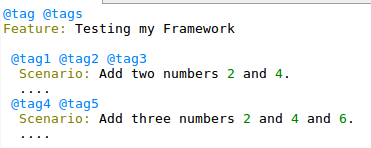
\includegraphics[]{tag.png}
	\caption{Tags}
	\label{rup6}
\end{figure}

A questão mais importante a se fazer ao identificar códigos e requisitos e tratar as associações de qual código pertence a qual requisito para uma eventual rastreabilidade.

{\textbf{Revisões para corrigir e identificar inconsistências:}} Atividade que deve ser feita periodicamente investigando os requisitos e o código que derivam desse requisito avaliando se este atende os pontos que foram propostos no requisito.

{\textbf{Gerenciamento de mudanças:}} O objetivo do gerenciamento de mudanças é garantir que os métodos e procedimentos padronizados mais adequados serão usados para o manuseio eficiente e imediato de todas as alterações. O objetivo é controlar a infraestrutura, a fim de minimizar o impacto de eventuais incidentes. Mudanças na infraestrutura de TI podem surgir de forma reativa em resposta a problemas ou exigências impostas externamente, por exemplo: alterações legislativas. Por outro lado, pode ser uma ação proativa de busca da maior eficiência e eficácia na organização.


\subsection{Gerência de Configuração GCO}

O proposito da Gerencia de Configuração é estabelecer e manter a integridade de todos os produtos de trabalho de um processo ou projeto e disponibiliza-los a todos os envolvidos.


Este modelo espera por 7 resultados em sua execução que serão tratados da seguinte forma:


{\textbf{Criação de um plano de gerenciamento de configuração:}} O plano deve identificar e mapear todos os itens de configuração que devem ser gerenciados e mantidos em uma baseline.


{\textbf{Identificação dos itens de configuração com base em critérios:}} Todo item que impactar nas configurações do produto ou projeto devem ser registrados em uma baseline.


{\textbf{Gestão das Baseline:}} A BaseLine é uma fotografia do projeto que deve ser tirada antes e depois de qualquer mudança esta deve conter todos os artefatos que foram alterados pela mudança, este registro histórico deve ser idêntico a o que esta descrito no projeto pois a não exatidão pode gerar uma não conformidade. Para controlar essas alterações foi utilizado o Git onde toda mudança foi evidenciada através de comentários e Tags.


{\textbf{Gerenciamento de Mudanças:}} Assim como nos requisitos a gerencia tem o objetivo de garantir que os procedimentos padrões serão adotados e seguidos da melhor maneira possível.


{\textbf{Auditorias de configuração:}} Trata-se de verificar se todos os itens que estavam planejados para o split foram atendidos e registrados devidamente nas Baseline, caso haja irregularidades estas devem gerar uma ou mais não conformidades que devem ser arquivadas e tratadas posteriormente.

\subsection{Garantia da Qualidade GQA}

O propósito é assegurar que os produtos de trabalho e a execução do processo estejam em conformidade com os planos, procedimentos e padrões estabelecidos.


Esta atividade possui 4 resultados esperados que pretende-se atender da seguinte forma:


{\textbf{Auditar os produtos de trabalho e os processos relacionados a projetos e processos organizacionais:}} Toda forma de trabalho ou processo dentro da organização pode eventualmente ser auditada em busca de prover melhoria a organização identificando falhas que podem estar contidas nela.



{\textbf{Registrar as não conformidades:}}As não conformidades devem ser registradas e priorizadas conforme sua criticidade, esta ação e simples e pode ser realizada através de um cheque list onde se verifica sé o modulo auditado esta produzindo os resultados esperados dentro do que foi proposto a ele. 
Após o registro um plano de ação deve ser elaborado afim de reduzir ou zerar os danos causados pela não conformidade afim de trazer melhorias a organização. 



{\textbf{Criar e acompanhar as ações corretivas para as não conformidades:}} Esta etapa se trata de garantir a qualidade do modelo de qualidade ou seja, devemos auditar o processo de qualidade afim de verificar se os planos de ações estão sendo executados se as não conformidades estão sendo relatadas e se o processo de qualidade esta sendo executado da maneira correta.


\subsection{Medição MED}

O proposito desta atividade e medir, coletar, armazenar e relatar os dados relativos aos produtos em desenvolvimento e os processos implementados na organização e em seus projetos, de forma a apoiar o objetivo da organização.


São 7 os resultados esperados que serão atendidos dentro dos seguintes processos:


{\textbf{Estabelecer metas de medição com base nos objetivos da empresa:}} Estabelecer um mapa estratégico, com a visão e a missão  da organização que irão nortear toda e qualquer métrica dentro do modelo.


{\textbf{Identificar e documentar medidas:}}Todos os processos devem ser estimados e cronometrados, afim de coletar as medidas resultantes da execução.


{\textbf{Coletar medidas, documental as e publicá-las: }} Estes dados devem ser expostos a todos da organização afim de buscar a melhora mutua de todos os processos setores e ativos. 


{\textbf{Executar ações decorrentes dos resultados:}} Esta e a mais importante das tarefas pois através dos resultados coletados e expostos pode-se traçar metas para se alcançar a melhoria dos resultados e observar desvios em estimativas incorretas que devem ser ajustadas para novos projetos. Essas ações podem ser realizadas a qualquer momento dentro do projeto isto depende muito do tamanho do projeto.


\subsection{Backlog e sprints}

    Fase de planejamento: O propósito desta fase é conseguir entendimento simultâneo entre todos os stakeholders (Gerente, Analista, Desenvolvedor) dos objetivos de ciclo de vida para o projeto, entender o que construir. Determine a Visão, o escopo do sistemas, organizações afetadas. Identifique quem é stakeholder (Cliente) do sistema assim como catalogar os riscos. Identifique as funcionalidades chave do sistema, decidir quais requisitos são mais críticos, determine pelo menos uma solução possível para os requisitos mais críticos. Identifique pelo menos uma arquitetura candidata para aplicação, entender os custos, cronograma, e os riscos associados ao projeto
Os projetos podem ter uma ou mais iterações na fase de planejamento. Entre algumas razões para ter múltiplas iterações na fase de planejamento, e que o projeto pode ser grande, e é difícil definir seu escopo. Sistema sem precedentes e muitos stakeholders (Cliente ou Organizações) com necessidades conflitantes e relacionamentos complexos. Grandes riscos técnicos que demandam a criação de um protótipo ou prova de conceito. A cada interação deve-se registrar uma baseline para armazenar um conjunto de itens de configuração que, normlalmente, representa o estado de desenvolvimento dos artefatos do projeto. A qualquer momento o gerente pode requisitar uma baseline histórica para  a utilização no projeto.
Quando o gerente assumir que o projeto não e viavel ou já não é mais lucrativo, este projeto deve ser encerrado seguindo o modelo do termo de encerramento de projetos, as partes devem ser comunicadas e a baseline deste projeto deve ser arquivada. 

 Modelo do processo BPMN figura \ref{rup3}: 
 \begin{figure}[h!]
    \centering
	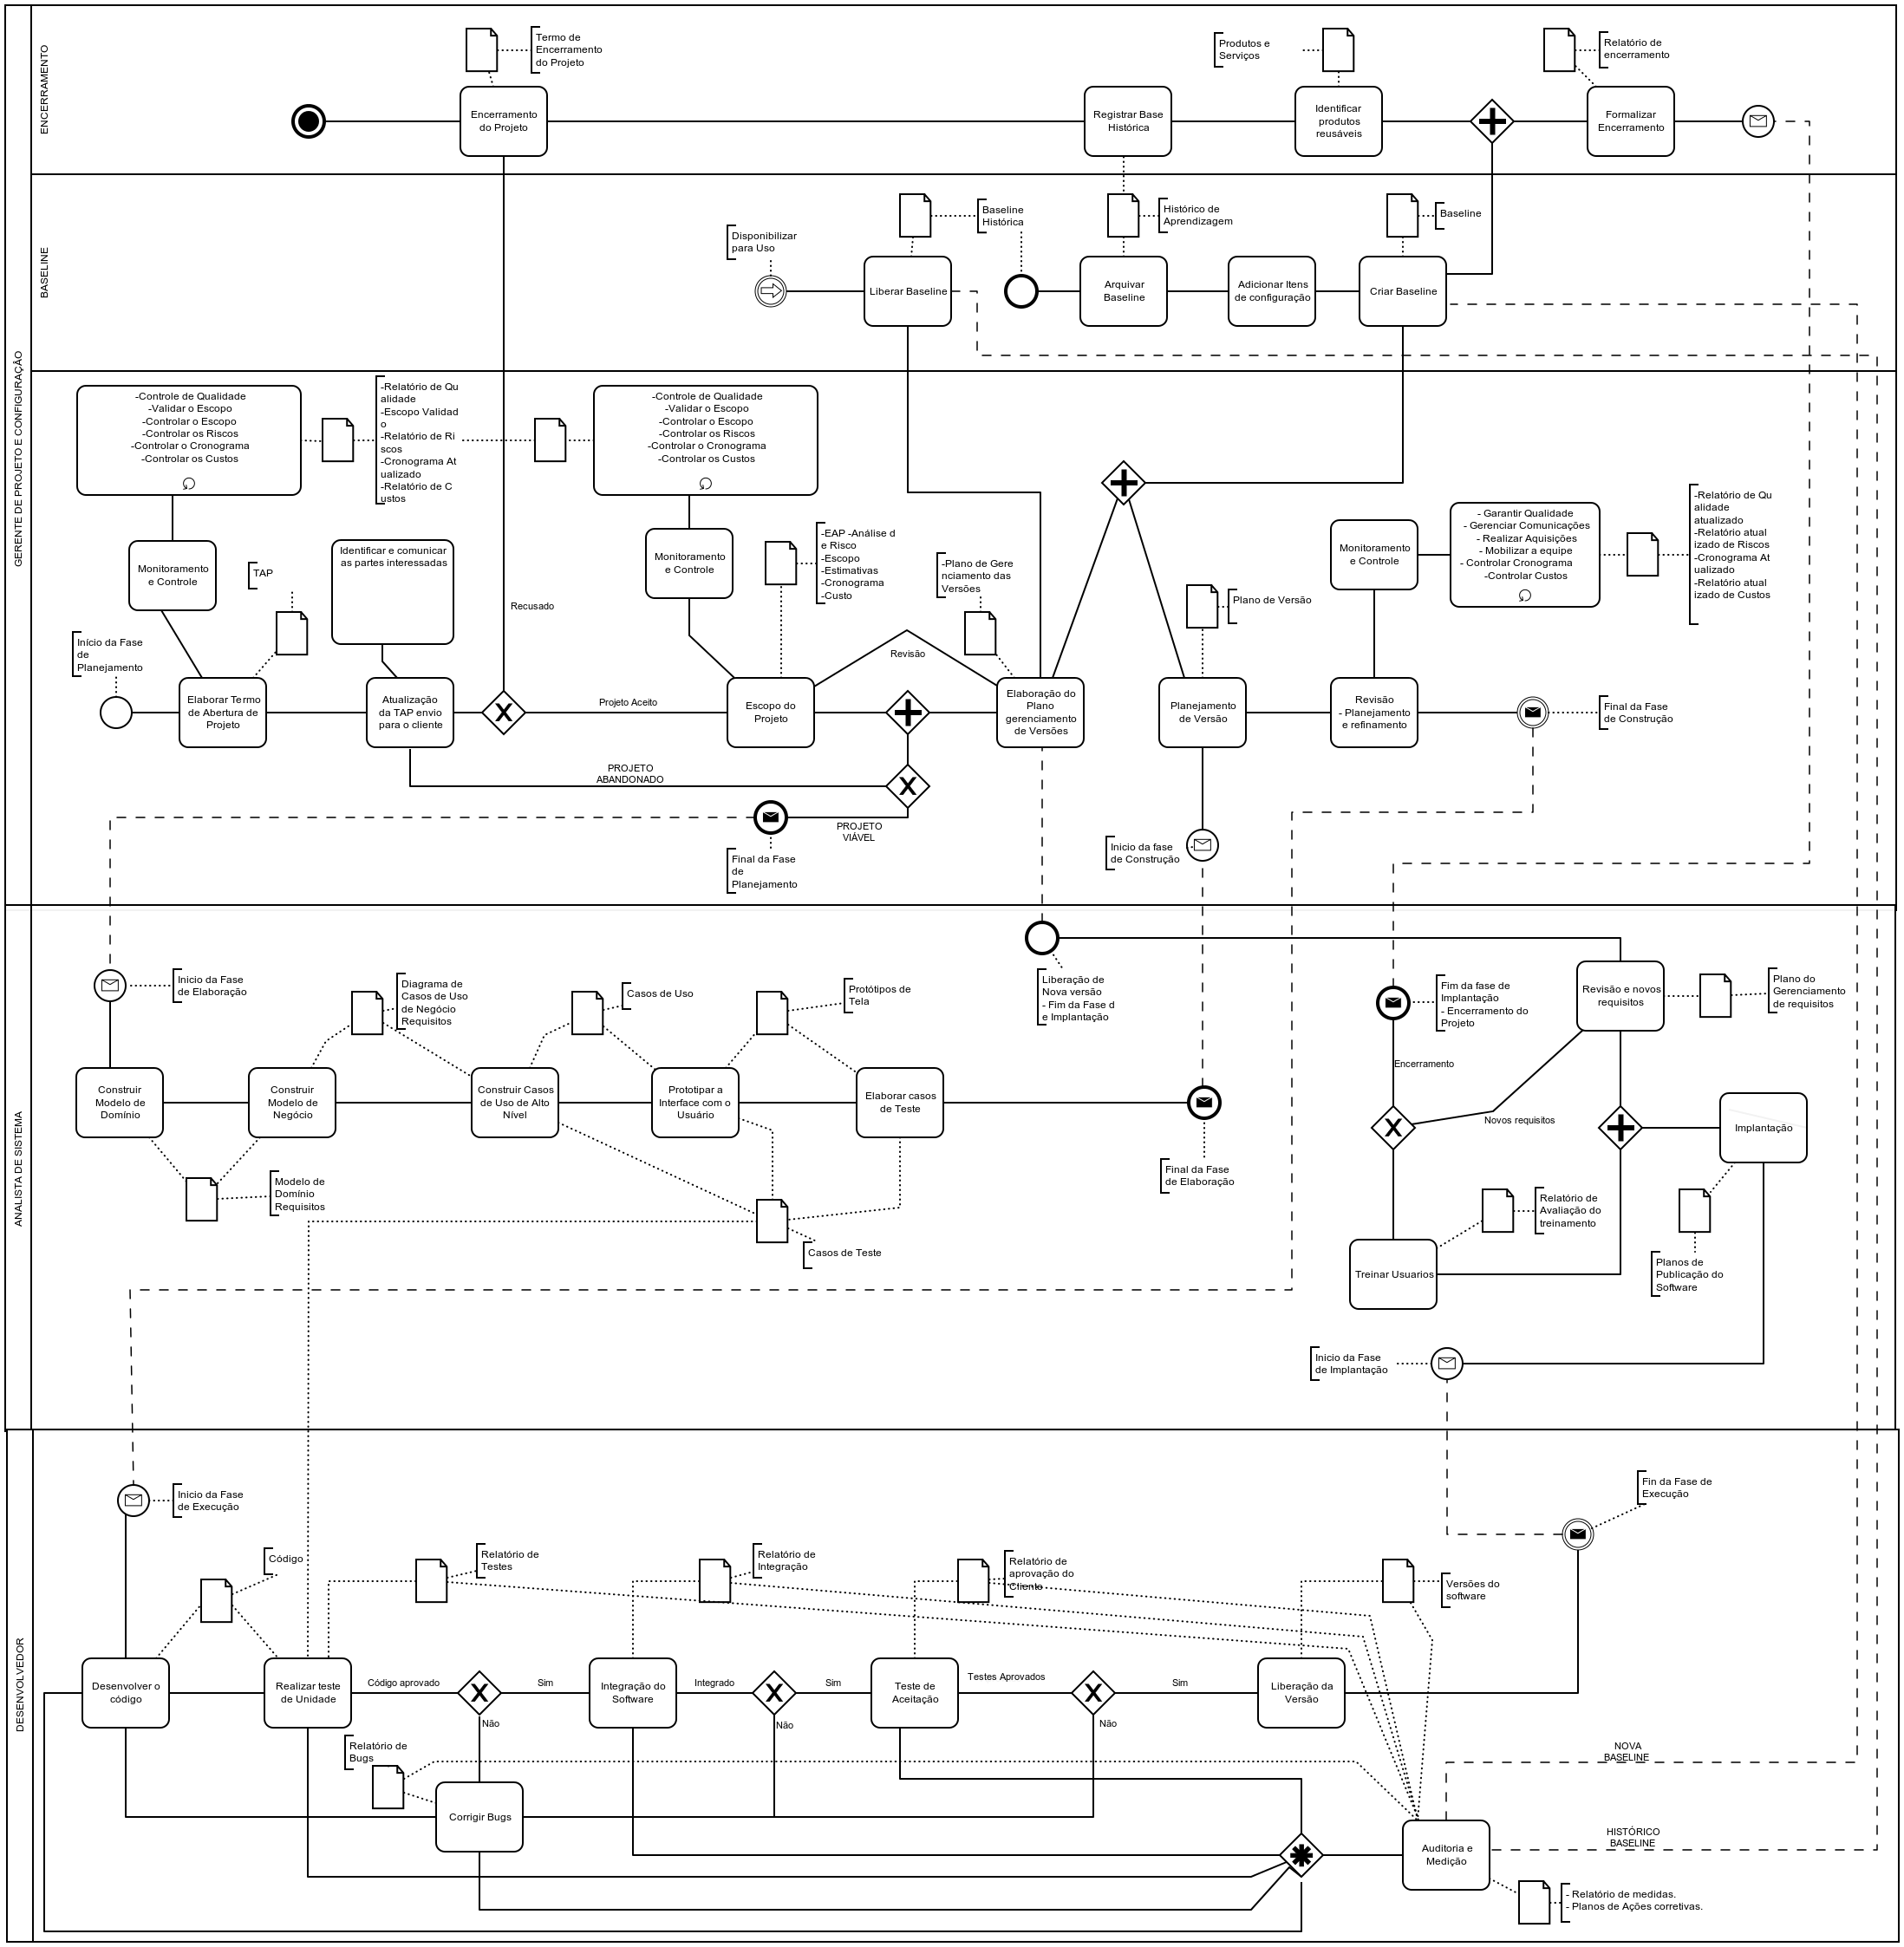
\includegraphics[scale=0.23]{diagramFinal.png}
	\caption{Processo BPMN}
	\label{rup3}
\end{figure}


Fase de Elaboração: O propósito desta fase é estabelecer uma linha de base da arquitetura do sistema e prover uma base estável para o backlog de esforço de desenvolvimento na próxima fase.
O objetivo desta fase e obter um entendimento mais detalhado dos requisitos. Com um bom entendimento dos principais requisitos de negocio e domínio permite a o Analista de sistemas criar um plano mais detalhado e obter comprometimento dos stakeholders (Cliente, desenvolvedor, Gerente do projeto). Um entendimento detalhado dos requisitos é essencial pois os críticos que serão validados serão implementados primeiro no splint Backlog. O analista Projetara, implementara casos de uso, validara unidades, projetara testes e estabeleça uma linha de base para a arquitetura. Apesar da funcionalidade não estar codificada ainda, a maior parte das interfaces de usuário entre os blocos sendo construídos. Estabelecemos aqui a nossa arquitetura inicial.
O número de iterações na fase de Elaboração é dependente de fatores como desenvolvimento de um novo produto a necessidade de manutenção do sistema, sistema sem precedentes versus tecnologia e arquitetura conhecidas, podem impactar no numero de interações.  A cada interação deve-se registrar uma baseline para armazenar um conjunto de itens de configuração que, representa o estado de desenvolvimento dos artefatos do projeto.

Fase de Construção: O Gerente do projeto deve minimizar os riscos essenciais e produzir um cronograma e uma estimativa de custos precisos. Muitos riscos técnicos são resolvidos como resultado do detalhamento dos requisitos e do projeto, implementação dos casos de uso, métricas e casos de teste. Refinar e detalhe o plano de projeto. Atualizar o plano da versão de acordo com o que foi coletado na fase anterior.
A fase de Construção tem mais iterações do que as outras fases, dependendo dos tipos de projetos projeto simples, uma iteração para construir o produto (para uma liberação beta) a partir desse ponto só se faz o controle e liberação das versões. Em projetos mais substanciais uma iteração para expor um sistema parcial e uma para amadurecê-lo para o teste beta. Projeto grande: Três ou mais iterações, dependendo do tamanho do projeto quantidade de requisitos  elevados para uma liberação beta. A cada interação deve-se registrar uma baseline para armazenar um conjunto de itens de configuração que, representa o estado de desenvolvimento dos artefatos do projeto.


Fase de Execução: Projetar, implementar, e testar um esqueleto da estrutura do sistema de acordo com a versão proposta pelo splint backlog são tarefas do Desenvolvedor. Apesar da funcionalidade não estar completa ainda, a maior parte das interfaces entre os blocos serão construídas é implementada e testada. Isto é conhecido como uma arquitetura executável. Na primeira iteração, o desenvolvedor deve projetar, implementar, e testar um pequeno número de cenários críticos para identificar que tipo de arquitetura e mecanismos de arquitetura serão utilizados para tratar o product backlog mais critico, atuando de acordo com o plano de versões onde os backlogs com maior alto grau de complexidade serão implementados primeiro. 
Nas próximas iterações, o desenvolvedor acata os requisitos coletados pelo analista e corrige o que não estava correto na iteração anterior. O desenvolvedor projeta, implementa, e testa os cenários significantes que restaram, garantindo que todas as áreas principais do sistema foram cobertas, tratando assim os riscos potenciais o mais rápido possível para entregar a versão aos stakeholders (Clientes). A cada interação deve-se registrar uma baseline para armazenar um conjunto de itens de configuração que, representa o estado de desenvolvimento dos artefatos do projeto.


Fase de Implantação: esta fase tem como objetivo assegurar que o software esteja pronto para ser entregue aos usuários.
Implantar o sistema Beta para validar se as expectativas dos usuários foram atendidas. Isto exige ajustes finos que podem gerar novos requisitos, tais como reparação de erros e melhorias no desempenho e na usabilidade. Obter a concordância dos stakeholders (clientes) de que a distribuição está completa. Isto pode envolver vários níveis de implantação para a aceitação do produto, implantações formais, informais e testes beta. 
A fase de implantação pode incluir a execução paralela de sistemas antigos e novos, migração de dados, treinamento de usuários e ajustes nos processos de negócio. A quantidade de iterações na fase de implantação varia de uma iteração para um sistema simples que necessita primeiramente de reparos de pequenos erros, até muitas iterações para um sistema complexo, envolvendo a adição de características e a execução de atividades para fazer a transição, no negócio, do uso do sistema antigo para o sistema novo. Quando os objetivos da fase de implantação são alcançados, o projeto está pronto para ser encerrado. O fim do ciclo de vida se encerra com a implantação da versão final do software no stakeholders (clientes). A cada interação deve-se registrar uma baseline para armazenar um conjunto de itens de configuração que, representa o estado de desenvolvimento dos artefatos do projeto.

\subsection {Versionamento}

 A modificação do produto exige que as alterações sejam salvas no Git, assim como registros de baseline. Para cada cliente deve-se criar uma nova branch de versionamento no Git, o nome da branch deve segir o modelo “branch\_ + versão do produto + Alteração”.
 
 
 Alterações que envolvam modificações no código ou correção de bugs devem ser destacadas nas @tags do git, lançado um incremento a versão de “1.0” para “2.0”.
 
 
Alteração de Layout e ajustes de documento dever ser destacadas nas @tags  do git, lançando um incremento na versão de “1.0” para “1.1”.  
  


Os requisitos alterados devem estar descritos no código através das @tags de controle assim como os requisitos a quais essas @tags atendem devem estar contidas no projeto.


Toda alteração no projeto seja de requisitos ou de código deve ser documentada no README.md, especificando de que maneira foi feito e por que foi feito.


Os requisitos para uma nova splint devem ser deixados anotados e documentados no README.md.  Assim qualquer membro pode dar sequencia no projeto.


Descrição das aterações no README \ref{rup12}: 
 \begin{figure}[h!]
    \centering
	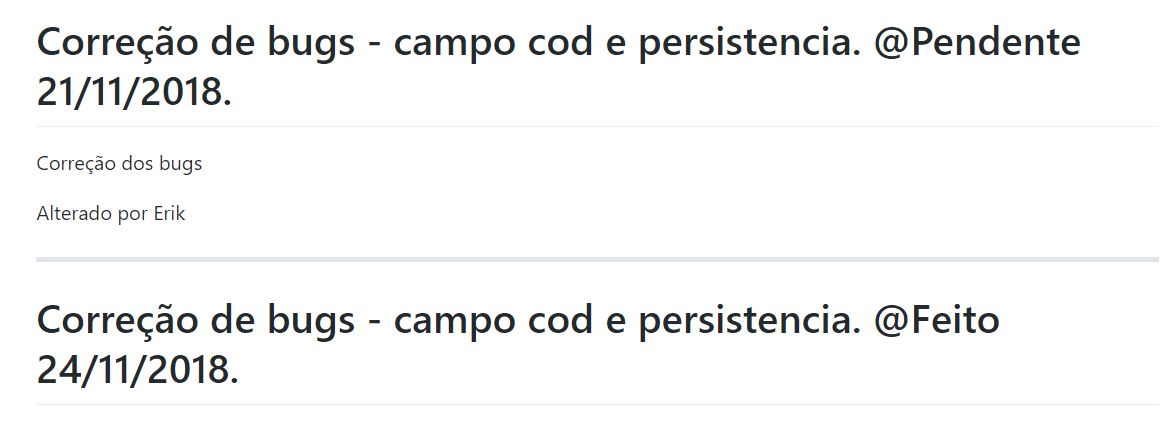
\includegraphics[scale=0.4]{readme.png}
	\caption{Versionamento README}
	\label{rup12}
\end{figure}

Os requisitos atendidos devem ser anotados com @Tags Concluido.


Quando o Projeto for Concluído deve-se destacar de forma clara ao final do documento do projeto em questão no arquivo README.md.

    
\subsection {Estado atual}

Artefatos gerados pelo processo em ordem cronológica tabela \ref{tab4}:
\begin{table}[h!]
\centering
\scalefont{0.9}
\caption{Tabela Cronologia dos Artefatos}
\label{tab4}
\begin{tabular}{|l|l|l|l|}
\hline
 & Artefato & Fase & Papel \\ \hline
1 & TAP & Planejamento & Gerente de Projeto e Configuração \\ \hline
2 & Relatorio de qualidade & Planejamento & Gerente de Projeto e Configuração \\ \hline
3 & Validação do Escopo & Planejamento & Gerente de Projeto e Configuração \\ \hline
4 & Relatório de riscos & Planejamento & Gerente de Projeto e Configuração \\ \hline
5 & Cronograma Atualizado & Planejamento & Gerente de Projeto e Configuração \\ \hline
6 & Relatório de Custos & Planejamento & Gerente de Projeto e Configuração \\ \hline
7 & EAP & Planejamento & Gerente de Projeto e Configuração \\ \hline
8 & Analise de Riscos & Planejamento & Gerente de Projeto e Configuração \\ \hline
9 & Escopo & Planejamento & Gerente do Projeto \\ \hline
10 & Estimativas & Planejamento & Gerente de Projeto e Configuração \\ \hline
11 & Cronograma & Planejamento & Gerente de Projeto e Configuração \\ \hline
12 & Custos & Planejamento & Gerente de Projeto e Configuração \\ \hline
13 & Gerenciamento de versões & Planejamento & Gerente de Projeto e Configuração \\ \hline
14 & Requisitos de Domínio & Elaboração & Analista de Sistemas \\ \hline
15 & Requisitos de Negocio & Elaboração & Analista de Sistemas \\ \hline
16 & Casos de Uso & Elaboração & Analista de Sistemas \\ \hline
17 & Protótipos de Tela & Elaboração & Analista de Sistemas \\ \hline
18 & Casos de teste & Elaboração & Analista de Sistemas \\ \hline
19 & Plano da Versão & Construção & Gerente do Projeto \\ \hline
20 & Relatório de qualidade & Construção & Gerente do Projeto \\ \hline
21 & Relatório de riscos atualizado & Construção & Gerente do Projeto \\ \hline
22 & Cronograma Atualizado & Construção & Gerente do Projeto \\ \hline
23 & Relatório de Custos atualizado & Construção & Gerente do Projeto \\ \hline
24 & Codigo & Execução & Desenvolvedor \\ \hline
25 & Relatório de Testes & Execução & Desenvolvedor \\ \hline
26 & Relatório de Interações & Execução & Desenvolvedor \\ \hline
27 & Relatório de Aprovação & Execução & Desenvolvedor \\ \hline
28 & Relatório de Bugs & Execução & Desenvolvedor \\ \hline
29 & Versões do Software & Execução & Desenvolvedor \\ \hline
30 & Relatório de Medidas & Execução & Desenvolvedor \\ \hline
31 & Plano de Ações & Execução & Desenvolvedor \\ \hline
32 & Publicação do Software & Implantação & Analista de Sistemas \\ \hline
33 & Gerenciamento de Requisitos & Implantação & Analista de Sistemas \\ \hline
34 & Treinamentos & Implantação & Analista de Sistemas \\ \hline
35 & Baseline & Presente em todas as Fase & Gerente de Projeto e Configuração \\ \hline
36 & Histórico de Aprendizagem & Presente em todas as Fase & Gerente de Projeto e Configuração \\ \hline
37 & Baseline Histórica & Presente em todas as Fase & Gerente de Projeto e Configuração \\ \hline
38 & Relatório de Encerramento & Implantação & Gerente de Projeto e Configuração \\ \hline
39 & Catalogo de Produtos Serviços & Implantação & Gerente de Projeto e Configuração \\ \hline
40 & Termo de Encerramento & Implantação & Gerente de Projeto e Configuração \\ \hline
\end{tabular}
\end{table}

\subsection{Boas Práticas}
\begin{itemize}

\item[1]  {\textbf{TDD - Test-Driven Development}}
O desenvolvimento orientado a testes é uma metodologia, que foi introduzida inicialmente pelo XP (Extreme Programming), a qual prega que os testes devem ser escritos antes da codificação. A escrita deve ser realizada pelo analista de sistemas e repassada ao desenvolvedor. A consequência disso é a possibilidade de alcançar total cobertura do código, uma vez que só o código a ser usado pelo teste deve ser escrito. Esta pratica e executada dentro do pacote de testes de aceitação do processo.

O fluxo de testes e dividido em 5 etapas:

    \item Planejar teste: o planejamento dos testes permite a identificação dos itens e funcionalidades que deverão ser testados, quem são os responsáveis e quais os riscos envolvidos, permite  definir o escopo, o custo e o prazo para as atividades de teste do projeto. Ainda na etapa de planejamento serão definidas estimativas, estratégias e técnicas de teste.
    
    \item Projetar teste: Com base nos requistos da funcionalidade o analista deve imaginar o fluxo de excução do componente elaborando um roteiro de testes automaticos. Com o documento escrito ele deve ser submetido aos testes.
    
    \item Executar teste: a execução do teste deve ser preferencialmente automática. Caso seja a primeira execução desse teste, necessariamente ele precisa falhar, uma vez que foi escrito antes da funcionalidade a ser implementada.

    \item Codificar: é a etapa na qual a funcionalidade será implementada pelo desenvolvedor, deve estar focada nos requisitos da funcionalidade, e apenas o código necessário para o teste ser executado com sucesso deve ser produzido.
    
    \item Refatorar código: nesse ponto o código produzido deve passar por uma "limpeza", com o objetivo de otimizar o código de maneira que seu comportamento não seja alterado. Uma vez realizada a refatoração do código, os testes automáticos devem ser executados para garantir que esta não inseriu erros no código da funcionalidade.

\item[2] {\textbf{Refatoração}}

Refatoração é o processo de alterar o código fonte de uma maneira que não altere seu comportamento externo e ainda melhore a sua estrutura interna. É uma técnica disciplinada de limpar e organizar o código, e por consequência minimizar a chance de introduzir novos. O uso desta técnica aprimora a concepção do sistema e evita a deterioração causada por mudanças com objetivos de curto prazo ou por alterações realizadas sem a clara compreensão do design do sistema. Além disso, o uso da refatoração durante o desenvolvimento do software facilitar o entendimento do código e sua manutenção.

\item[3] {\textbf{Ciclo de vida Scrum}}

O primeiro passo é definir a visão do produto com base em informações colhidas junto ao usuário final, equipe, stakeholders e gerentes; nesta etapa será criada pelo Gerente e o Analista uma lista inicial de todos os itens que devem ser produzidos no decorrer do projeto para que a visão do produto seja bem sucedida, essa lista é denominada de product backlog. Uma vez que existe o product backlog o produto será desenvolvido através de iterações conhecidas como Sprints. 

   A equipe de desenvolvimento planejam o Sprint, essa reunião é chamada de Planning Meeting, e é divida em duas partes: a parte tática e a parte técnica. Na parte tática o Gerente deve fazer os ajustes necessários para o Product Backlog e em sequência definir a meta do Sprint. Após a definição da meta o time deve selecionar os itens com os quais podem se comprometer. Na parte técnica o time deve se reunir para tomar as decisões de como fazer cada item do Product Backlog, isso será feito através da quebra de tarefa, depois o time deve estimar cada tarefa para averiguar a viabilidade do desenvolvimento da mesma, o resultado da parte técnica é o artefato chamado Sprint Backlog. Ou seja, o Sprint Backlog é uma lista de requisitos, assim como o product backlog, porém reduzida para que possa ser efetivadas dentro do Sprint. Para uma melhor visibilidade do projeto o Sprint Backlog pode ser representado em forma de quadro Scrum.

    Agora pode-se iniciar o Sprint, que deve ser feito pela equipe de desenvolvimento de acordo com o tempo estimado, realizando Daily Scrum todos os dias dando origem a um ciclo menor. Ao termino do Sprint é realizado uma reunião de Review. Seu objetivo é apresentar o que foi realizado.

    Por fim, após a reunião de Review é realizada uma ultima reunião do Sprint, que muitos acreditam ser a mais importante, a Retrospectiva. O seu objetivo é levantar os pontos bons e ruins do Sprint. Finalizando a retrospectiva retorna para o Planning Meeting, dando início ao ciclo maior.
    
    \item[4] {\textbf{Planning Poker}}
    
O Planning Poker é uma técnica de estimativa baseada no consenso de toda a equipe, onde é utilizado um conjunto de cartas com valores específicos, praticado como se fosse um jogo. Essa técnica foi descrita pela primeira vez em 2002, por James Grenning, e foi popularizada depois por Mike Cohn no livro Agile Estimating and Planning.

\end{itemize}

\section{Projeto Produto Inova}

\subsection{Distribuição do Produto}

Para a distribuição conforme o necessário, foi criado um repositório no GuitHub onde o produto original assim como as demais versões são armazenados,  assim podendo replicar em diversos usuários através do comando “git clone”, onde o repositório máster será clonado, as demais versões podem ser acessadas através do comando ”git checkout”, alternando entre branchs, pode-se acessar as diferente versões do produto.

   Ate o momento o processo atende a três clientes, que podem acessar as diferentes distribuições através do VNC Viewer.

\begin{itemize}

\item As distribuições para acesso remoto dos clientes estão distribuídas da seguinte maneira:

\item[0] Servidor Linux ip: 10.20.19.13
\item Senhas para accesso: abc123
\item[1] Porta de acesso cliente\_1: 10.20.19.13:7
\item Senhas para accesso: abc123
\item[2] Porta de cesso cliente\_2: 10.20.19.13:3
\item Senhas para accesso: abc123
\item[3] Porta de acesso cliente\_3: 10.20.19.13:4
\item Senhas para accesso: abc123
\item[4] Porta de acesso cliente\_4: 10.20.19.13:6
\item Senha para accesso: abc123
\end{itemize}

\subsection{Manutençaõ Servidor}

Novas distribuições para acesso remoto podem ser cridas acessando o servidor linux e seguindo as instruções.

Deve-se acessar o IP 10.20.19.13 através do protocolo ssh.
O logim do super usuário é: utfpr – senha: abrobinha.

Para cada cliente atendido e necessário a criação de um novo usuário no servidor.

Atualmente o servidor possui três usuários:
\begin{itemize}
\item Usuário: Cliente 1 – Login cliente\_1 – Senha: abrobinha.
\item Usuário: Cliente 2 – Login cliente\_2 – Senha: abc123.
\item Usuário: Cliente 3 – Login cliente\_3 – Senha: abc123.
\item Usuário: Cliente 4 – Login cliente\_4 – Senha: abc123.
\end{itemize}



\subsection{Versões Produzidas}
(Ao clicar na brnach desejada o link com o repositorio do GhuitHub ira abrir):

\begin{itemize}

\item O produto inicial está armazenado no repositório:
\href{https://github.com/ErikZA/ProdutoInova/tree/master}{ErikZA/ProdutoInova}


\item Foi criado uma brach denominada \href{https://github.com/ErikZA/ProdutoInova/tree/branch_V1_Original}{branch\_V1\_Original}, esta base armazenara os dados da versão do produto que será disponibilizada ao clientes 1.

\item A base  \href{https://github.com/ErikZA/ProdutoInova/tree/branch_V1_Original}{branch\_v1\_Original\_2}, esta base armazenara os dados da versão do produto que será disponibilizada ao clientes 2.

\item Uma brach denominada \href{https://github.com/ErikZA/ProdutoInova/tree/branch_V2_LayoutRed}{branch\_V2\_LayoutRed}, esta base armazenara os dados da versão do produto que será disponibilizada ao cliente 3.


\item A base \href{https://github.com/ErikZA/ProdutoInova/tree/branch_V3_PersistenciaUF}{branch\_V3\_PersistenciaUF}, esta base mantem os dados do produto que será disponibilizado para o cliente 4.


\end{itemize}

\subsection{Atualização}

O processo de atualização e executado da quando o produto instalado no cliente sofrer alterações em sua base online no GitHub, quando esta nova versão estiver disponível deve-se realizar o comando “git pull” na maquina do cliente, o produto de software deve ser novamente construído e executado para utilizar as novas funcionalidades.

\section{Referências bibliográficas}
\renewcommand\refname{} %%Referências bibliográficas}  
\bibliographystyle{ieeetr}
\begin{itemize}

\item The Unified Process Explained - Book by Kendall Scott.
\item Um Guia do Conhecimento Em Gerenciamento de Projetos - Guia Pmbok® - 5ª Ed. 2014 - Institute, Project Management.
\item Métodos Ágeis em Gerenciamento de Projetos - Rafael Dias Ribeiro,MSc,CSM,CSPO,ACP,PMP. Horácio da Cunha e Sousa Ribeiro,MSc.
\item Processo Demoiselle v1.2.3b -	https://www.frameworkdemoiselle.gov.br/

\item Desenvolvimento agil: http://www.desenvolvimentoagil.com.br/scrum

\item Noções de Engenharia de Software: http://nocoesengsw.blogspot.com/2010/03/stakeholders.html

\item Dissciplinas do Processo Unificado: http://jkolb.com.br/disciplinasfases-processo-unificado/

\item Modelo de qualidade MPS'BR:
https://www.softex.br/mpsbr/

\item TDD simples e prático:   https://www.devmedia.com.br/test-driven-development-tdd-simples-e-pratico/18533


\end{itemize}
\bibliography{referencias}  

%% ***********************************************************************
\end{document}
